\documentclass[twocolumn,12pt]{article}

\usepackage{amssymb}%Blacksquare
\usepackage[margin=0.7in]{geometry}
\usepackage{amsmath,parskip,graphicx} 
\usepackage[utf8]{inputenc} %not clear effect
\usepackage[T1]{fontenc} %not clear effect
\usepackage[english]{babel}% not clear effect
\usepackage{float} %used for fixed tables with [H]
\usepackage[document]{ragged2e} %used to justify text
\usepackage{amsthm}
\usepackage{commath}
\usepackage{textcomp}
\usepackage{enumerate}
\usepackage{wrapfig}
\usepackage{cite}
\usepackage{amssymb}
\usepackage{epstopdf}
\usepackage{inputenc}
\usepackage{array}
\usepackage{booktabs}
\usepackage{subfig}
\usepackage[justification=centering]{caption}
\usepackage{array}% http://ctan.org/pkg/array	
\usepackage[nottoc]{tocbibind}
\usepackage{breqn} %used to split equations on multiple lines
\usepackage{listings}
\usepackage{pdfpages} %used to include pdfs
\usepackage{mhchem} %used for writing chemical reactions
\usepackage[justification=centering]{caption}
\usepackage{array}% http://ctan.org/pkg/array	
\usepackage[nottoc]{tocbibind}
\usepackage{fancyhdr} %doing header and footer
\usepackage{tikz} %initializing the package
\usetikzlibrary{calc}

%commands used for code inserting
\usepackage{listings}

\definecolor{dkgreen}{rgb}{0,0.6,0}
\definecolor{gray}{rgb}{0.5,0.5,0.5}
\definecolor{mauve}{rgb}{0.58,0,0.82}

\lstset{frame=tb,
  language=Java,
  aboveskip=3mm,
  belowskip=3mm,
  showstringspaces=false,
  columns=flexible,
  basicstyle={\small\ttfamily},
  numbers=none,
  numberstyle=\tiny\color{gray},
  keywordstyle=\color{blue},
  commentstyle=\color{dkgreen},
  stringstyle=\color{mauve},
  breaklines=true,
  breakatwhitespace=true,
  tabsize=3
}

\usepackage{array}

\usepackage{titlesec}
\usepackage[titletoc,toc,title]{appendix} %used for apendix

\usepackage{multicol} %used for multiple columns


\newcommand\numberthis{\addtocounter{equation}{1}\tag{\theequation}} %usec to number equations in multi-line unmbered environment, e.g. in align* 
\numberwithin{equation}{section} %used to number equations per section as wel
\DeclareMathOperator\erf{erf} %defining erf function


\usepackage{hyperref} %Used to hyper reference.Usually it has to be the last package to be imported, but there might be some exceptions to this rule.



\restylefloat{table}
\numberwithin{equation}{section}

\title{University Physics Competition - 2017}
\author{The best team}
\date{\today}   

\pagestyle{fancy}
\fancyhf{}
\lhead{Magnetic lens grid}
\chead{University Physics Competition}
\rhead{Team 825}
\cfoot{Page \thepage}

\renewenvironment{abstract}{
\begin{center}
\begin{minipage}{0.85\textwidth}
\rule{\textwidth}{0pt}}
{\par\noindent\rule{\textwidth}{0pt}
\end{minipage} \end{center}}

\begin{document}

\begin{titlepage}
\begin{center}
\vspace{5mm}
\huge{Reducing ion beam divergence using a magnetic lens grid} \\
\vspace{5mm}
\Large{Team 825: Problem B Ion Thrusters} \\
\vspace{5mm}


\textbf{Abstract:}\\
\vspace{5mm}
\end{center}

\begin{abstract}
\justify
Divergence of the ion beam thrusters may extend over wide angles, significantly decreasing the thrust. The proposal that magnetic fields may be used is thoroughly investigated from ion production to final exhaust before neutralizer. The distribution of ions positions and velocities is analyzed and a theoretical maximal improvement of $\approx 10$\% was deduced. Another grid using magnetic lenses was introduced using non-homogeneous magnetic field was used to make the ion paths more uniform. The focal length of such lens is inversely proportional to the intensity of the magnetic field, numerically a focal length of the lens of 2.5m with coil current of 0.0033A with 2500 number of turns was obtained. Furthermore, a simulation of the behaviour of Xenon ions from jet thruster was presented. It was concluded that it is not practical to introduce such magnetic lenses, as no significant improvement could be achieved.

\end{abstract}
\end{titlepage}
\newpage



\tableofcontents

\justify

\section{Introduction}

Ion thrusters have proven to be a successful system for propelling space probes through our solar system. Having been not the only electric thruster method discovered so far (e.g. arcjets, hall thrusters, pulse jets, etc.), gridded electrostatic ion thrusters begin by ionizing their propellant, accelerating the positively charged ions using a potential difference between two or more grids, and then neutralizing the exhaust by firing a beam of electrons into it. In the present paper, the divergence of the outgoing ion beam is thoroughly investigated to conclude whether generating a magnetic field that would affect the trajectories of ions out of the final grid to collimate the ions brings a significant improvement. At a first sight, under the (ideal) physical models that assume symmetry and homogeneity, this proposal deems itself highly unpractical and inefficient. However, taking a closer look at perturbations and non-homogeneous aspects, one discovers significant divergence effects which could be reduced by a magnetic field. 

This paper is organized as follows. In section \ref{backgroundinformation}, the relevant information regarding ion thruster optics is reviewed, focusing on the position and angle of the ions in the beam. The position is approximated by a bi-modal normal distribution and the angle increases linearly with the distance from the centre of the aperture. In section \ref{magneticlenssection}, the magnetic lens theoretical analysis was carried out. Section \ref{technicalities} deals with practical limitations and engineering considerations for designing a grid consisting of magnetic lenses. An ion jet for one aperture was simulated and analyzed under different parameters. Its simulation is open to the public under the following link: . In section \ref{sectionconclusion}, a summary of strengths and weaknesses was presented. Since space-travel is a very interesting problem, section \ref{sectionfurtherresearch} was dedicated to discuss further improvements, focusing on ion beam manipulation using magnetic fields. 

Throughout the document, the theoretical consideration are put into practice for a prototype Xenon ion thruster, with $R_t=35$ cm in diameter, with a specific impulse of $ I_{sp} = 5 100$ s and a thrust of $T = 350$ mN. Wherever not explicit, it is always had in mind how can this be feasible.

\begin{figure*}
    \centering
    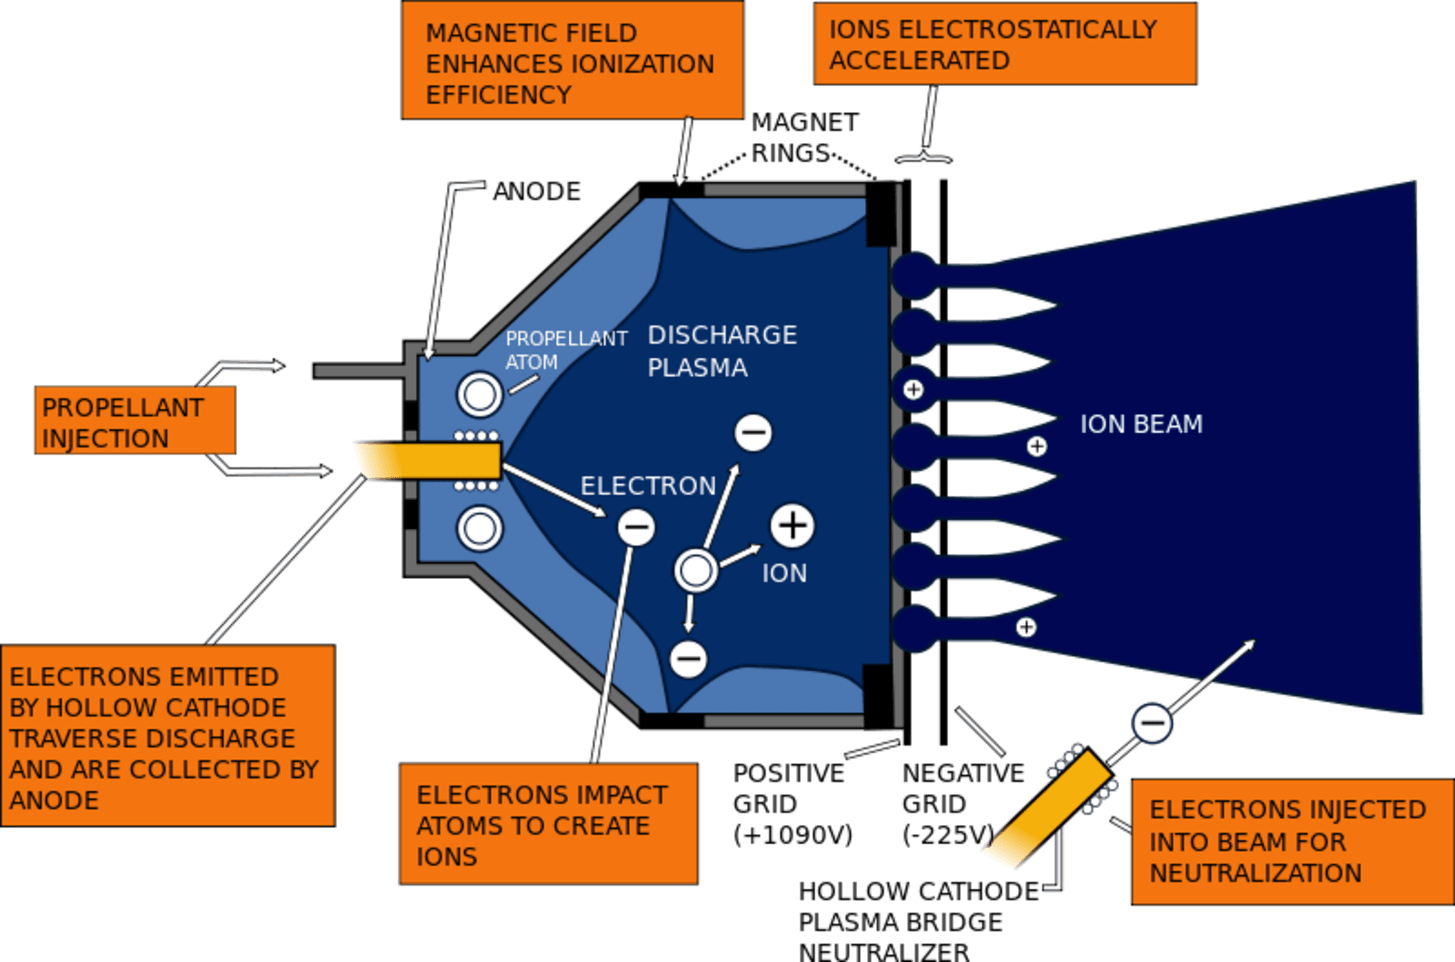
\includegraphics[width=0.75\textwidth]{figs/ionthruster.png}
    \caption{Ion Thruster Operation \cite{nasa} showing the ion accelerator, the plasma generator, and the neutralizer cathode}
    \label{ionthruster}
\end{figure*}

\section{Background information for Ion Thruster Optics}
\label{backgroundinformation}
Ion thrusters are characterized by the electrostatic acceleration of ions extracted from the plasma generator \cite{kaufman}. Multiple techniques for ionization can be used, the most common one is electron bombardment (illustrated in case of direct current (DC)  in Fig. \ref{ionthruster}), followed by contact ionization, radio-frequency ionization, and others. The ion accelerator consists of (at least two) electrically biased multi-aperture grids, assembly called the ion optics. The electrical scheme (Fig. \ref{electricalschemewithgrids}) together with the positive ions motion (Fig. \ref{motioninsidegrids}) depict the sought behaviour for an ideal jet. 

The grids consists of smaller apertures through which the ion jets pass and form the ion beam. To roughly summarize: the screening grid selects the positive ions and "reflects" the electrons; the acceleration grid evidently accelerates the ions; the third (optional) deceleration grid protects the acceleration grid from corrosion. This reasoning is explained further in Ref. \cite{mitcourse}, and more detailed in Chapter 5 of Ref. \cite{fundamentalsofelectricpropulsion}.
\vfill
\begin{figure}[H]
    \centering
    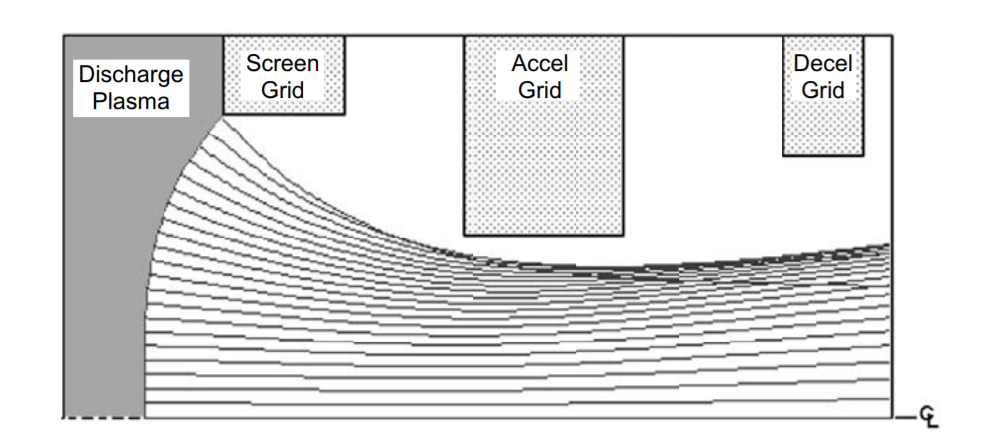
\includegraphics[width=0.5\textwidth]{figs/motioninsidegrids.PNG}
    \caption{Ion trajectories from a plasma sheath (on the left) in a half-beamlet inside an example three-grid accelerator\cite{fundamentalsofelectricpropulsion}}
    \label{motioninsidegrids}
\end{figure}


\begin{figure}[H]
    \centering
    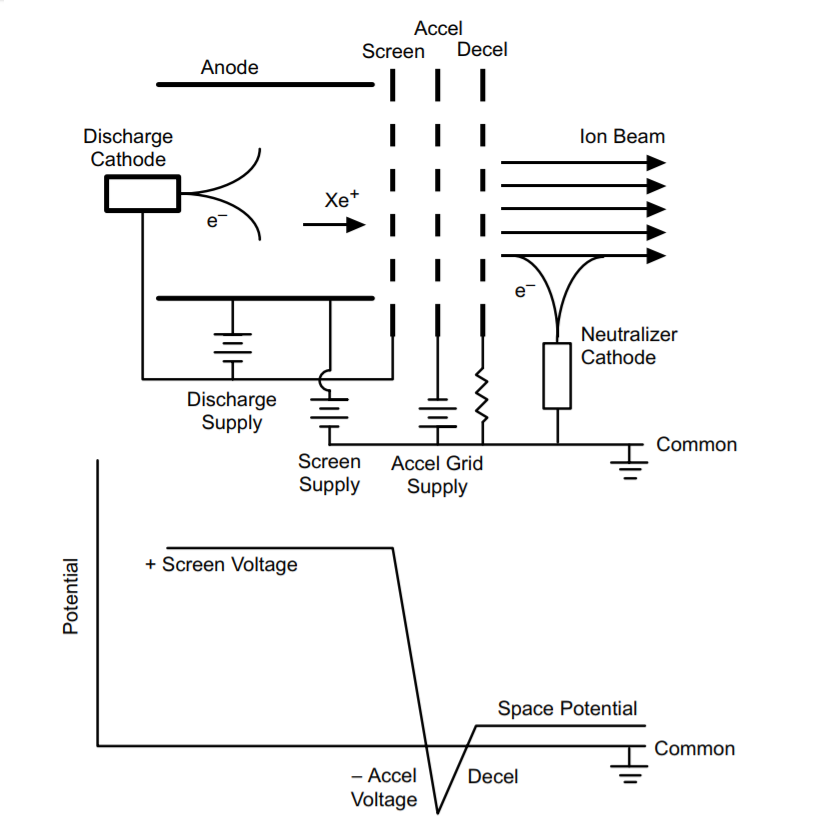
\includegraphics[width=0.5\textwidth]{figs/Grids.PNG}
    \caption{Electrical scheme of a DC discharge with three grids \cite{fundamentalsofelectricpropulsion}}
    \label{electricalschemewithgrids}
\end{figure}


\subsection{Thrust}
The thrust  supplied by the engine to the spacecraft can be easily derived. Here, the derivation of Ref \cite{fundamentalsofelectricpropulsion}, chapter two is followed. The spacecraft mass decreases with time due to the propellant mass $m_p$ consumption, hence the thrust $T$ is given by the time rate of change of the momentum:
\begin{equation}
T = \dfrac{d}{dt}(m_p v_{ex}) = \dot{m}_p v_{ex} \approx \dot{m}_i v_i
\end{equation}
where the exhale velocity $v_{ex}$ is the ion constant velocity after acceleration in the potential $V_b$, whence $v_i = \sqrt{2 q V_b/M}$. It was assumed that after being ionized in the electron bombardment chamber, the positive gas ions diffuse in the screen grid region and get accelerated uniformly, i.e. all ions have the same velocity $v_i$, but with slightly different orientations. The beam current $I_b$ is related to the mass flow rate $m_i$ of ions with mass $m$ by:
\begin{equation}
    \dot{m}_i = \dfrac{I_b m}{q}
\end{equation}
which can be used to give the thrust as:
\begin{equation}
    T = \sqrt{\dfrac{2M}{e}} I_b \sqrt{V_b} 
\end{equation}
However, this assumed an ideal collimated jetbeam. A simple correction factor $\gamma = F_t \cdot \alpha$ can be considered to be made of a factor $F_t$ taking into account the divergence of the beam and another term $\alpha$ that accounts for the presence of multiply charged ion species.

The usual propellant gas used in Ion (and Hall) thrusters is Xenon, for it is an heavy inert gases (does not react with the space craft elements). Moreover, its properties are marvelously explained in \cite{fundamentalsofelectricpropulsion}, Chapter 1: "it is not hazardous to handle and process, it does not condense on spacecraft components that are above cryogenic temperatures, its large mass compared to other inert gases generates higher thrust for a given input power, and it is easily stored at high densities and low tank mass fractions." Then, the total thrust for Xenon (with $\sqrt{2M/e} = 1.65 \cdot 10^{-3}$ can be written as:
\begin{equation}
    T = 1.65 \cdot 10^{-3} \gamma I_b \sqrt{V_b}
\end{equation}
In this paper, one is interested only in the beam divergence and how it can be improved, i.e. how can thrust increase by reducing the wasted ion momenta in the perpendicular direction to the motion of the rocket.

In our model, the thrust and specific impulse necessary was 0.35N and 1500 seconds respectively. Since, the specific impulse expression is given by:
$I_{sp}=\frac{T}{\dot{m_p}g}$, where $I_{sp}$ is the specific impulse, $\dot{m_p}$ is the mass-flow rate, and $g=9.807m/s^2$ is the acceleration due to gravity on earth surface.
This gives value of mass flow rate to be around 23.8 mg/s. With the mass of Xenon, one can obtain the no.of Xenon ions flowing outside of thruster per second to be around $1.09 /cdot 10^{-20}$. Finally, combining with the expression for the thrust, one can obtain the speed of ions coming outside of the accelerator grid to be around $1.473 \cdot 10^4 m/s$.

\subsection{Position and velocity distribution of individual ions in the ion beam}
\label{distribution}

For the present treatment, the main effect to be taken into consideration is the ions distribution of position and velocities which produce the thrust. Under the proposal that ions exit the final grid at a wide range of angles, it is of uttermost importance to understand how they are produced in first place. Already carried out by different groups and available in the scientific literature, a great deal of computer simulations have been reviewed, also in the attempt to understand erosion \cite{erosion}, life-time \cite{lifetime1} \cite{lifetime2}, high specific impulse behaviour \cite{highspecificimpulse}. Based on these results, an approximation for the distribution is now derived.

The physical processes are highly complicated and several papers have been written using different assumptions. Two representative results from the literature are presented in Figures \ref{model1pic} and \ref{model2pic}. The latter is particularly interesting, as it takes into account charge exchange(CEX) ions to the grid erosion in an electron bombardment ion thruster. This deviates considerably from the collision-less case, because it deviates (diverges) ions in regions otherwise empty.

\begin{figure}[H]
    \centering
    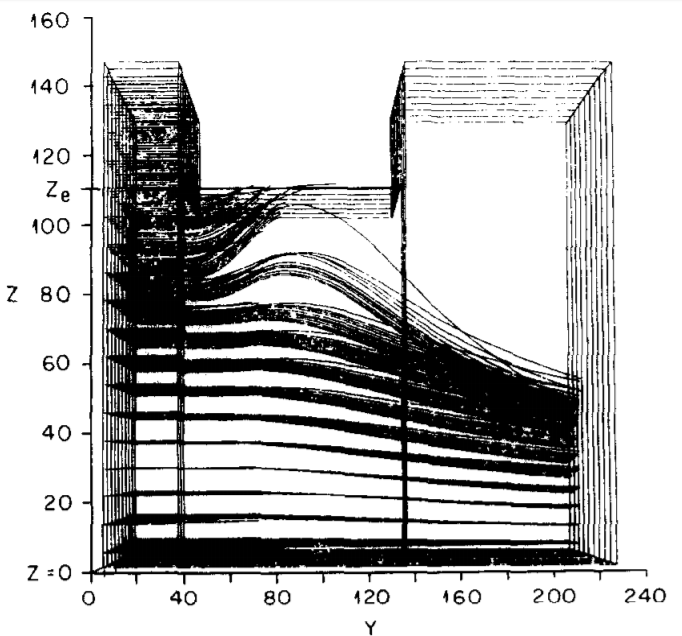
\includegraphics[width=0.5\textwidth]{figs/model1.PNG}
    \caption{Ions trajectories in three-grids ion thruster \cite{model1ref}}
    \label{model1pic}
\end{figure}

\begin{figure}[H]
    \centering
    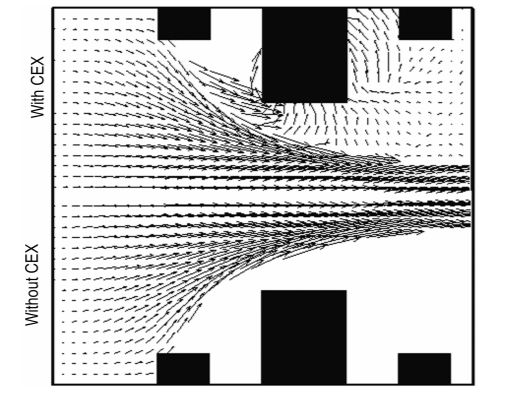
\includegraphics[width=0.5\textwidth]{figs/model2.PNG}
    \caption{Comparison of ion velocity vector distribution (Top: with charge exchange collision, bottom: without) \cite{lifetime1}}
    \label{model2pic}
\end{figure}

The approximate model is considered to be a mixture  of two Gaussian Random Variables distributions (see Appendix \ref{randomvariables} for clarifications), equally shifted from the center of the aperture with radius $a$, i.e. a bimodal distribution. This graphically resembles a ring with decaying edges or a valey sorounded by hills. Appendix \ref{appendixnumerical} is dedicated to the numerical computations using the online version of WolframAlpha \cite{wolframalpha} or, internally, the Sympy Package of Python 3.6.  The result of this section is equation \ref{finalequation}. To not interrupt the reading flow, the reader interested only in its consequences can skip its explicit derivation. Here, the Gaussians are centered at $\mu_{1,2} = \pm a/4$ with the same standard deviation $\sigma_1 = \sigma_2=\sigma = a/4$, giving the final normalized distribution as:
\begin{equation}
    f(r) \approx \dfrac{4}{a} \sqrt{\dfrac{2}{\pi}}\left[ e^{-\dfrac{(4r+a)^2}{2 a^2}} + e^{-\dfrac{(4r-a)^2}{2 a^2}} \right]
    \label{finaldistribution}
\end{equation}
where $r$ is the distance from the center of the aperture. The weak equality sign is used to provide a better equation in terms of readability of coefficients, but in the explicit computations the strict sense using all factors which are very close to 1 ($\approx 1$, e.g. \ref{approxexample}).

Only the 1D model was discussed, which suffices for both analytical and simulation taks, because of the rotational symmetry of the jet beam. Consider a 2D distribution $f(x,y) = z$. Given any point $(x,y)$, the cross-section along the line defined by the origin $O = (0,0)$ and $(x,y)$ is identical for any choice of $x$ and $y$. Hence, one changes to cylindrical coordinates where only one parameter (the radius) plays a role.

\begin{figure}[H]
    \centering
    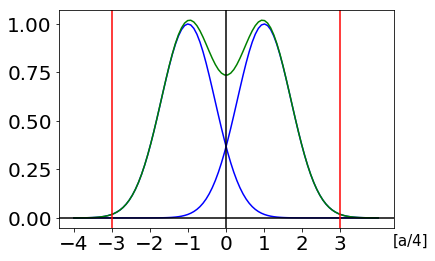
\includegraphics[width=0.5\textwidth]{figs/twogaussians.png}
    \caption{Two RVs model in 2D where the z-direction is suppressed. Note that in 3D, this is similar to a "donut" hole distribution, with the remark that the centre is not empty.  More than 95\% can be found inside the red lines (placed at $-3a/4$ and $+3a/4$) }
    \label{RVdistribution}
\end{figure}

A very useful formula to compute the divergence correction factor for cylindrical thrusters is given in Ref \cite{fundamentalsofelectricpropulsion}, chapter two:
\begin{equation}
    F_t = \frac{1}{I_B}\int_0^a  2 \pi r J(r) \cos \theta(r) dr
    \label{correctionfactor}
\end{equation}

Two cases are identified, on whether $\cos \theta(r)$ is constant or not. 


\subsubsection{Constant $\cos \theta (r) = \cos \theta$}
Due to the intrinsic randomness, one may consider a constant deflection angle (with respect to $r$). The current distribution $J(r)$ for one aperture is then:
\begin{equation}
    J(r) = \dfrac{I_b}{A} f(r)
\end{equation}
which gives via equations \ref{finaldistribution} and \ref{correctionfactor}:
\begin{equation}
    F_t =  0.990 \cdot \cos \theta
    \label{constantthetasolution}
\end{equation}
For a decently collimated jet beam with thrust half angle of 10 deg, the correction factor becomes $F_t = 0.99 \cdot \cos\theta = 0.975$, which represents a 2.5\% loss in thrust. At first sight, it seems unreasonable to mount an extra grid only for such a small correction, but (!) one further assumes wide range of angles. The decay of the thrust is then $\sim \cos \theta$, which is unacceptable: e.g. for a thrust half angle 45 deg, the correction factor becomes $F_t = 0.7$, a 30\% loss in thrust! However, this is under the assumption that the angle does not depend on the position of the ions. From Figures \ref{model1pic} and \ref{model2pic}, this is clearly a very rough approximation.

\subsubsection{Varying $\cos \theta(r) = \cos \alpha \dfrac{r}{a}$}
\label{varyingtheta}
One assumes a model where the deflection angle increases (linearly) with the distance $r$ from the centre of the aperture, as suggested by the aforementioned papers and figure. Hence, one tries an approximation of the form:
\begin{equation}
\cos \theta(r) = \cos \alpha \dfrac{r}{a}
\end{equation}
where $\alpha$ is a parameter related to the maximal angle of deflection, in particular:
\begin{equation}
    \alpha = \theta_m
\end{equation}
Note that at the margins, one obtains $\cos \theta (r=a) = \cos \theta_m$, as expected. The integral of \ref{correctionfactor} then becomes:
\begin{equation}
    \int_{0}^{+a} dr \cdot r f(r) \cos \alpha \dfrac{r}{a} 
    \label{complicatedintegral}
\end{equation}

Unfortunately, this does not yield a suitable solution after integration and further numerical analysis using Taylor series was carried out, as explained in Appendix \ref{appendixnumericalb}. The correction factor then becomes:
\begin{equation}
    F_t(\alpha) =   2 \cdot ( 0.497 - \dfrac{0.122}{2!} \alpha ^2 + \dfrac{0.0468}{4!} \alpha^4)
    \label{finalequation}
\end{equation}
which for $\theta = 45^{\circ} = \pi/4$ rads gives $F_t = 0.915$, a much more realistic result. This model can be further improved by analyzing more physical phenomenon and by considering a random noise. Furthermore, one may consider a non-linear formula for the angle, i.e. $\theta = f(r)$, such as Gaussian centered at the origin, exponential decay after a certain radius, etc. Considering the neglected effects, the maximum improvement one hopes for is $~15\%$.

Now, one may restrict their considerations only to a single aperture, if the magnetic field is identically applied to each aperture; or to consider a total distribution for N (usually a couple of thousands) aperture. Here, the former is analyzed, as implemented via magnetic lenses. 


\subsection{Reasons for beam divergence}
In the theoretical model, the beam jets behave smoothly and only their divergence is given by the ion production in the gas chamber and deviations due to the applied magnetic fields. In practice, several physical effects and mechanical defects cause deflections:
\begin{enumerate}
    \item Misalignment of the grid apertures causes off-axis deflection of the ion trajectories, named beam steering\cite{misalignment1} \cite{misalignment2}.
    \item Misalignment of the grids themselves deflecting the jet beam.
    \item Coulomb interaction among ions and the electrons.
    \item Charge-Exchange Collisions (only briefly mentioned in Figure \ref{model2pic}.
    \item The effect of the introduced magnetic field, as it is not only confined inside the magnetic lenses.
\end{enumerate}

\section{Magnetic lens}
\label{magneticlenssection}
One can think of using homogeneous magnetic field to deflect the diverging particles with wide angles, but due the nature of Lorentz's force, one cannot use it to solve the problem. Suppose two ions with different angles enters a magnetic field at the same position. Since they have different angles with respect to the magnetic field, when one corrects angle for one ion, the other ion will change the angle. While correcting the angle for other, the one with correct angle will change. Thus, it is not possible to correct both ions with the same homogeneous magnetic field. This is shown in \ref{ionmotion1} and \ref{ionmotion2}. The graph is obtained by modifying \cite{code} such that the individual trajectories is changed. 

\begin{figure}[H]
    \centering
    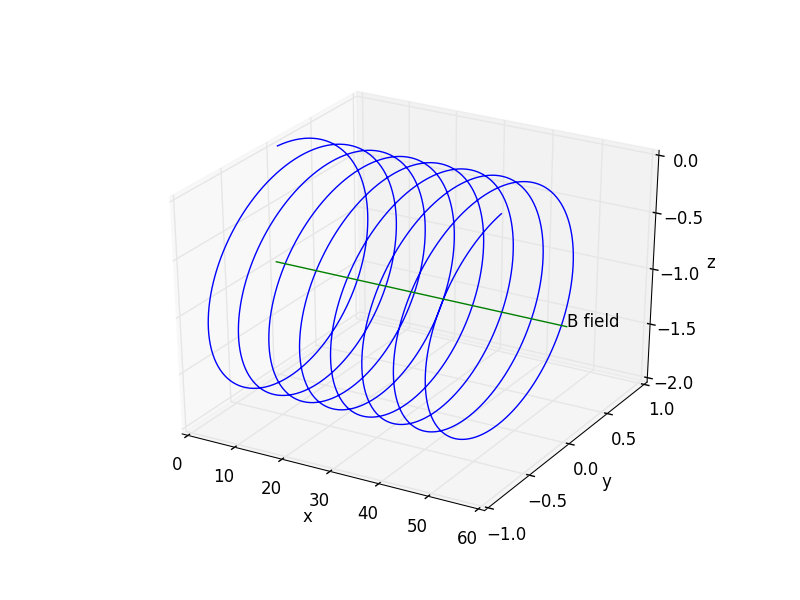
\includegraphics[width=0.5\textwidth]{figs/ionmotion1uniform.png}
    \caption{Motion of ion in uniform magnetic field with velocity vector = 0.05}
    \label{ionmotion1}
\end{figure}
\begin{figure}[H]
    \centering
    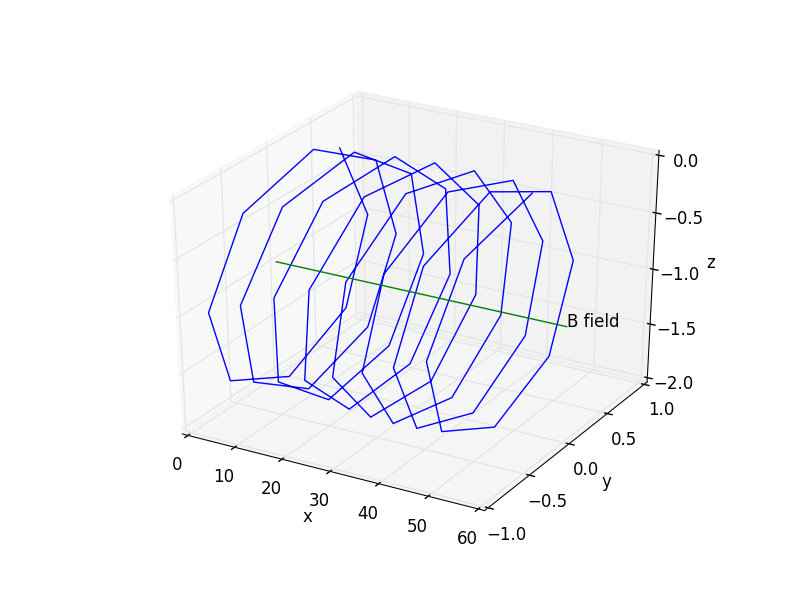
\includegraphics[width=0.5\textwidth]{figs/ionmotion2uniform.png}
    \caption{Motion of ion in uniform magnetic field with velocity vector = 0.8}
    \label{ionmotion2}
\end{figure}
It can be clearly seen in \ref{ionmotion1} and \ref{ionmotion2}  that even though both ions have same position, they follow completely different path due to their different velocity component. This makes it impossible to direct large number of ions with multiple angles to an uniform direction. 
figure \ref
Other approach would be using time varying magnetic fields so that one can trap the wide angled ions while releasing the linear angled ions. Repeating this step continuously will eventually give out the linear angled ions. Even though this approach sounds promising, it is very difficult to solve it as this case will involve solving three dimensional time varying magnetic fields which includes second order partial differential equations coming from Lorentz's and Newton's equation. Solving it numerically would also be very expensive. 

Another approach is to use to  magnetic lenses on each aperture which would represent a fourth grid that could be inserted even before the deceleration grid.
Magnetic lens is a device used for deflecting charged particles with magnetic field. Magnetic lens are used in several devices such as Electron microscope, particle accelerators, cathode tubes and so on. In general, when a charged beam of diverged particles are passed through the magnetic lens, it comes out converged on the other side. Focal length of such magnetic lens is dependent on the magnetic fields applied and ion current. \cite{booktheory} Focal length for a strong magnetic field is shorter while focal length for weaker magnetic fields is longer. One can use this property to find a uniform direction ion beam when ion beams with wide angles are entered. 

\begin{figure}[H]
    \centering
    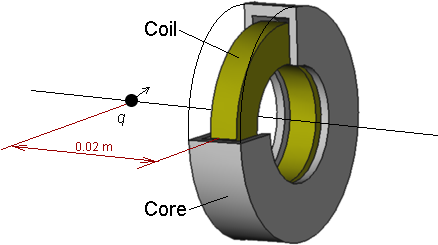
\includegraphics[width=0.5\textwidth]{figs/magnetic_lense_model.png}
    \caption{Model of magnetic-lens \cite{maglens}}
    \label{maglen}
\end{figure}

\subsection{Assumptions for analysis}
Inside the laboratories in Earth, magnetic lenses are operated in vacuum. Fortunately space can be assumed as a perfect vacuum, so the calculation were based in vacuum. Relativistic effects were ignored even though ions emerging outside of the accelerator grid has a very high speed. Though, two positively charged ions interact with each other due to Coulumb's force, it was assumed that there is no interaction among themselves in the calculation. 


\subsection{Behavior of ions in Non-uniform magnetic fields}
As magnetic field problems require three dimensional geometry to find the solution, it is often difficult to find an analytic solution except for certain limiting cases. In many cases, the magnitude of the velocity remains constant when subjected to the magnetic field alone\cite{booktheory}, but the direction of the ions changes substantially. Combining Newton's law of motion and Lorentz's force in the Cartesian coordinates give following sets of differential equation:
\begin{align*}
    \frac{m}{q} \frac{d^2x}{dt^2}&=B_y\frac{dz}{dt}-B_z\frac{dy}{dt}\\
    \frac{m}{q} \frac{d^2y}{dt^2}&=B_z\frac{dx}{dt}-B_x\frac{dz}{dt}\\
    \frac{m}{q} \frac{d^2z}{dt^2}&=B_x\frac{dy}{dt}-B_y\frac{dx}{dt} \numberthis{}
    \label{cartesiancoord}
\end{align*}

where $m$ is the mass and $q$ the charge of the ion, $B_i$ components of the magnetic field. Exploiting the rotational symmetry of the magnetic lens, one can use cylindrical coordinates to rewrite the above differential equations in a more suitable form. In cylindrical coordinate system, $(r, \theta,z)$ component represent radial distance, angle and axial distance respectively, which in terms of the cartesian coordinates $(x,y,z)$, can be written as:
\begin{equation}
    r=\sqrt{x^2+y^2} \quad     \theta= \tan^{-1}\frac{y}{x} \quad    z=z
\end{equation}
With the above, one can obtain the following set of differential equations in cylindrical coordinates:
\begin{align*}
    \frac{m}{q}\left(\frac{d^2r}{dt^2}-r(\frac{d \theta}{dt})^2\right)= B_\theta \frac{dz}{dt}- B_z\frac{rd\theta}{dt}\\
    \frac{m}{q}\left(\frac{1}{r}\frac{d}{dt}(r^2\frac{d\theta}{dt})\right)=B_z\frac{dr}{dt}-B_r\frac{dz}{dt}\\
    \frac{m}{q}\frac{d^2z}{dt^2}= B_r \frac{rd \theta}{dt}- B_{\theta}\frac{dr}{dt}
    \label{setofdiffeq  } \numberthis
\end{align*}
In equations \ref{setofdiffeq}, the left hand side terms represents components of acceleration in $r$, $\theta$ and $z$ direction and fully describe the motion of ions in Non-uniform magnetic field. 

The path of ions in non-uniform magnetic field is shown in \ref{ionmotion3}. The graph is modified from \cite{code} by making Electric field 0 and changing trajectories for individual particles. 
\begin{figure}[H]
    \centering
    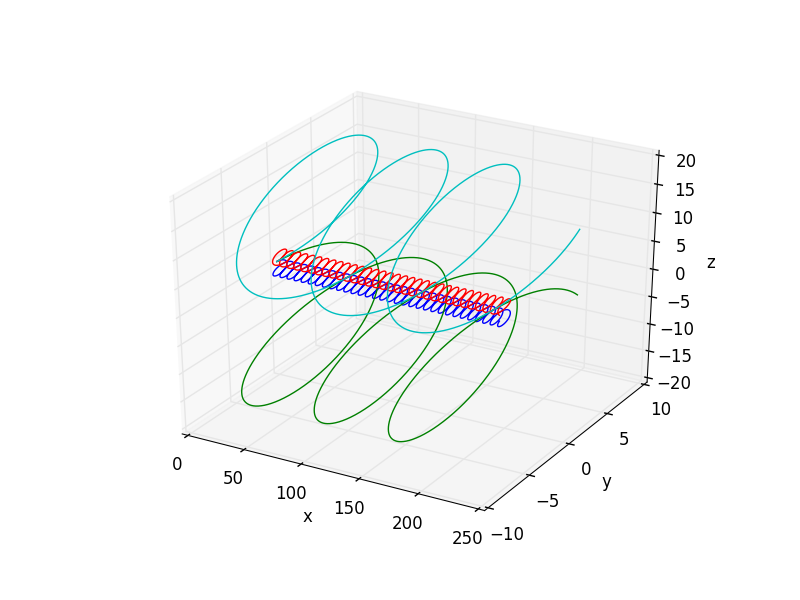
\includegraphics[width=0.5\textwidth]{figs/motion of ions nonuniform.png}
    \caption{Motion of ions in non-uniform magnetic field( weak in the centre, strong in the boarders), Particles passing through the centre goes un-deflected, while particles in the boundary goes deflected}
    \label{ionmotion3}
\end{figure}

\subsection{Properties of magnetic lensing}
Focal length of the magnetic lens depends upon several parameters such as axial component of velocity, lens voltage, magnetic field intensity of the magnetic lens at different positions and so on. In general, Focal length of the magnetic lens is directly proportional to the x-component of the velocity ($f \propto v_x$) and inversely proportional to magnetic flux density ($ f  \propto 1/ B$).\cite{designmaglens} It will be later shown that path of ions coming out of the lens is always converging. In our model, we wanted an uniformly straight path of ions which can be obtained if the focal point of the lens is ideally at infinity i.e it converges at infinity. This can be obtained by applying relatively weak magnetic field in the lens coil and analyzing other necessary parameters. 


Charged particles such as ions or electrons move in a straight line, and when they experience magnetic field short uniformly parallel to axis, it gains angular component of the force. This happens because radial component of the velocity reacts to the axial component of the magnetic flux. This will cause the flow of charged particles such as ions or electron to twist their path. As they twist, angular $\theta$ component reacts with the axial component of the field. This causes radial component of the force directed towards path. Thus, the charged particles such as ions or charges follow the path of the magnetic fields and come out of the lens as defined by the focal length of the lens. \cite{maglenstheory}

\subsection{Rotational symmetry approach}
It is well known that every component of the magnetic field satisfies Laplace's equation. If one applies Laplace's equation for the axial component of the magnetic flux, we get following set of the differential equation:
\begin{align}
    \frac{1}{r} \frac{\partial }{\partial r} \left (r \frac{\partial B_z}{\partial r} \right )+ \frac {\partial ^2 B_z}{\partial z^2}=0
    \label{diffeq}
\end{align}
Partial differential equation \ref{diffeq} can be solved by power series technique as follow:
\begin{align}
    B_z(r,z)= B_0- \frac{r^2}{4}B_0^{''}+ \frac{r^4}{64}B_0^{''''}+ ...
    \label{powerseries}
\end{align}
where, $B_0=B_z(0,z)$
Equation \label{powerseries} can be written tightly in a summation form as:
\begin{align}
    B_z(r,z)=\sum_{n=1}^\infty (-1)^{n+1} \left(\frac {r}{2} \right)^{2n-2} \frac{B_0^{2n-2}}{[(n-1)!]^2}
\end{align}

\subsection{Ions motion in magnetic fields: cylindrical coordinates}
Applying Maxwell's equation $\nabla \cdot B =0$, 
we get: 
\begin{align}
\frac {1}{r} \frac {\partial}{\partial r}(rB_r) + \frac{\partial B_z}{\partial z}=0 
\label{Maxwell}
\end{align}
Applying \ref{diffeq} to \ref{powerseries}, one can obtain:
\begin{align}
B_r= \sum{n=1} ^\infty \frac{(-1)^nr^{2n-1}B_0^{2n-1}}{2n[(n-1)!]^22^{2n-2}}
\end{align}
% Ion motion in magnetic field expressed by cylindrical coordinates:
Lorentz's force states that force on a moving charged particle with velocity $\vec{B}$ only in a magnetic field $\vec{B}$ is given by:
\begin{align}
\vec{F}=q(\vec{v} \times \vec{B})= m \vec{a}
\label{Lorentz}
\end{align}
Writing \ref{Lorentz} in component form, yields the following set of differential equations:
\begin{align*}
    \frac{m}{q}[\ddot{r}-r\dot{\theta}^2]=B_\theta \dot{z}- B_zr\dot{\theta}\\
    \frac{m}{q}\frac{1}{r}\frac{d}{dt}(r^2\dot{\theta})= B_z\dot{r}-B_r\dot{z}\\
    \frac{m}{q}\ddot{z}=B_rr\dot{\theta}-B_{\theta}\dot{r} \numberthis
    \label{NLComp}
\end{align*}
If one has magnetic field with rotational symmetry then, $B_\theta=0$. Above equations simplifies further if one uses approximation by ignoring $r^2$ terms. \cite{booktheory}
Integrating for the angle $\theta$, gives:
\begin{align}
    \dot{\theta}=\frac{q}{m} \frac{B_0}{2} + C
    \label{theta}
\end{align}
Integration constant $C$ becomes zero as angular velocity is zero when magnetic field is zero. Applying \ref{theta} to find the radius yields:
\begin{align}
    \ddot{r}=-r\left(\frac{q}{m}\frac{B_0}{2}\right)^2
    \label{r..}
\end{align}
Again using \ref{r..} to find the height, one gets $\ddot{z} =0$ which is correct up to first order. 


If one again approximate axial component of the velocity as the ion's velocity i.e. $v=\dot{z}$ and approximate $\ddot{r}=\dfrac{2Vq}{m}\dfrac{d^2r}{dz^2}$ with $V= \dfrac{mv^2}{2e}$, after substituting in \ref{r..}, the second order ordinary differential equation is obtained:
\begin{align}
    \frac{d^2r}{dz^2}+ \frac{q}{8mV} B_o^2r=0
    \label{ionpath}
\end{align}
This equation describes the path of ions in the presence of non-homogeneous magnetic field, so is important for analyzing focusing properties of lens. This Ordinary differential equation can be solved exactly. Define all the constant as $C=\frac{qB_o^2}{8mV}$, then the differential equation turns into 
\begin{align}
    \frac{d^2r(z)}{dz^2}+ Cr(z)=0
\end{align}
The general solution can be obtained by defining $m^2=-C$, $m=\pm \sqrt{C}i$ with $p=0$ and $q=\sqrt{C}$.
The general solution is now: 
\begin{align}
    r(z)=e^{pz}(P\cos(qz)+Q\sin(qz))
\end{align}
Since $p=0$ and $q=\sqrt{C}$,one can obtain the solution of the above differential equation as:
\begin{align}
    r(z)=Pcos(\sqrt{C}z)+Qsin(\sqrt{C}z)
    \label{pathion}
\end{align}
Since \ref{pathion} is second order differential equation, given initial conditions, \ref{pathion} describes the path of ion when they move inside the magnetic lens at any angle. In this case, required initial conditions are $r(0)$ and $d/dz(r)|_0$ where $r(0)$ gives information about position of ion and $d/dz(r)|_0$ gives information about the angle made by ions while passing through the lens. 

\subsection{Magnetic lens focusing}
Equation \ref{ionpath} can be used for obtaining the focal length of the magnetic lens for thin magnetic field. When one does that, one can get Busch equation\cite{Electrmic} of focal length as:
\begin{align}
    \frac{-1}{f_2}=\frac{q}{8mV} \int_{z_1}^{z_2}B_o^2dz
    \label{focal}
\end{align}
In \ref{focal}, $z_1$ and $z_2$ indicates the start and end point of magnetic lens. 
For a magnetic lens of a radius R with N number of circular turns of wire with I current flowing through wire:
\begin{align}
    B_0=\frac{\mu _o I R^2 N}{2(R^2+z^2)^{3/2}}
    \label{circwire}
\end{align}
In order to calculate focal length of magnetic lens, one need to compute the integral:
\begin{equation}
I_1=\int_{z_1}^{z_2} \left(\frac{1}{(R^2+z^2)^{3/2}}\right)^2dz
\end{equation}

This can be solved by substituing method:
\begin{equation}
z=R\sinh x \quad dz=R\cosh x dx \quad z^2=R^2\sinh^2x
\end{equation}
Now, the integrand becomes,
\begin{align}
    I_1=\int_{x_1}^{x_2}\frac{R\cosh x}{(R^2+R^2\sinh^2x)^3}dx =                 \frac{1}{R^5}\int_{x_1}^{x_2}\cosh^{-5}x dx
    \label{I1}
\end{align}
The solution of focal length for such a magnetic field is given by\cite{booktheory}:
\begin{align}
    f=\frac{97.9VR}{I^2}
\end{align}
For coil with N, number of turns and certain coil factor $c_F$ is then,
\begin{align}
    f=\frac{97.9VR}{(NI)^2} \cdot c_f
    \label{focal}
\end{align}
If one plot \ref{focal}, one will get,

\begin{figure}[H]
    \centering
    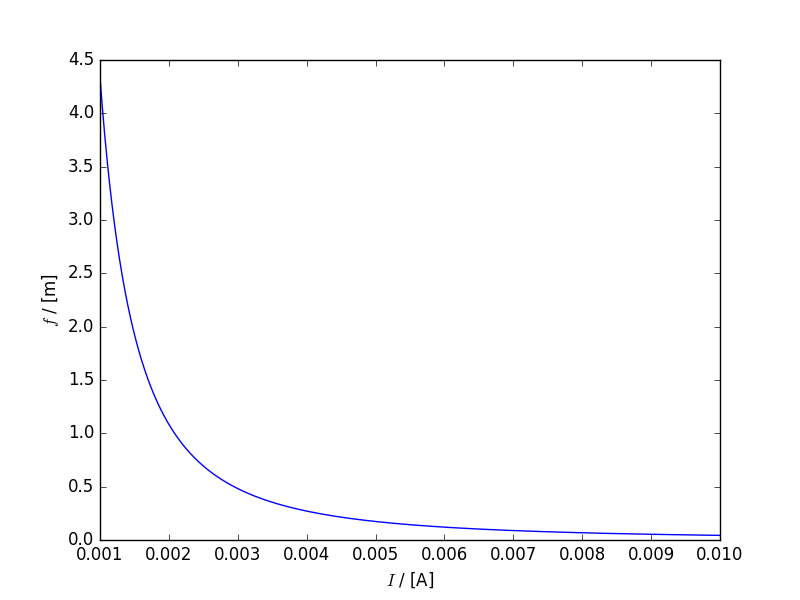
\includegraphics[width=0.5\textwidth]{figs/focal length, current relation.png}
    \caption{Model of magnetic-lens \cite{maglens}}
    \label{focal}
\end{figure}

Fromm the graph \ref{focal}, one can see that focal length increases with decreasing coil current. At coil current 0.0033A, one can see that focal length will be around 2.5m. This shows that the ion beams that comes out diverged from the accelerator grid will gets converged after very long distances. Thus, they can be approximated as an uniform. 

The figure depicting the flow of ions from the apperture and outward from the lens is shown in 
\begin{figure}[H]
    \centering
    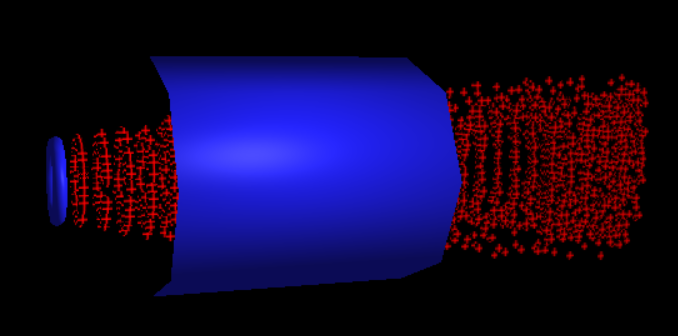
\includegraphics[width=0.5\textwidth]{results/Simulation.png}
    \caption{Magnetic lens in working}
    \label{focal}
\end{figure}

\section{Technical considerations for the Ion thruster}
\label{technicalities}
Depicted in Fig. \ref{aperturegridspic}, the grids consist of smaller apertures with radius $a$ typically in range of 1 to 5 cm. The number and area of the apertures, as well as the distance between them play a significant role in the ion beam output. Each small aperture behaves like described in section \ref{distribution}, and their 3D sum yields the ion beam in Figure \ref{ionthruster}. In this section, the technical implementation is investigated. The aperture radius was considered to be $a = 1.25$ mm. To find the number $N_a$ of apertures considering the a hexagonal lattice (as in Fig. \ref{aperturegridspic}) for the structure of apertures (rectangular centered could have been considered as well) such that the distance between the centers of two adjacent apertures is $d = 4$ mm > $2.5$ mm $= 2a$ (aperture diameter), one finds that $N = \frac{\pi R_t^2}{d ^2} \approx 6 000$ apertures. Since each lens is designed to act on only on aperture, one has the same number of lenses $N_l = N_a$. The lens are designed of around 10 cm with focal length of 2.5m. From, /ref{focal}, we obtained that coil current need to be around 0.0033A for converging the beams at the distance of 2.5m.If necessary, one can also play with current and magnetic field variables to change the focal length of the lens so that the beams comes uniform. 

\begin{figure}[H]
    \centering
    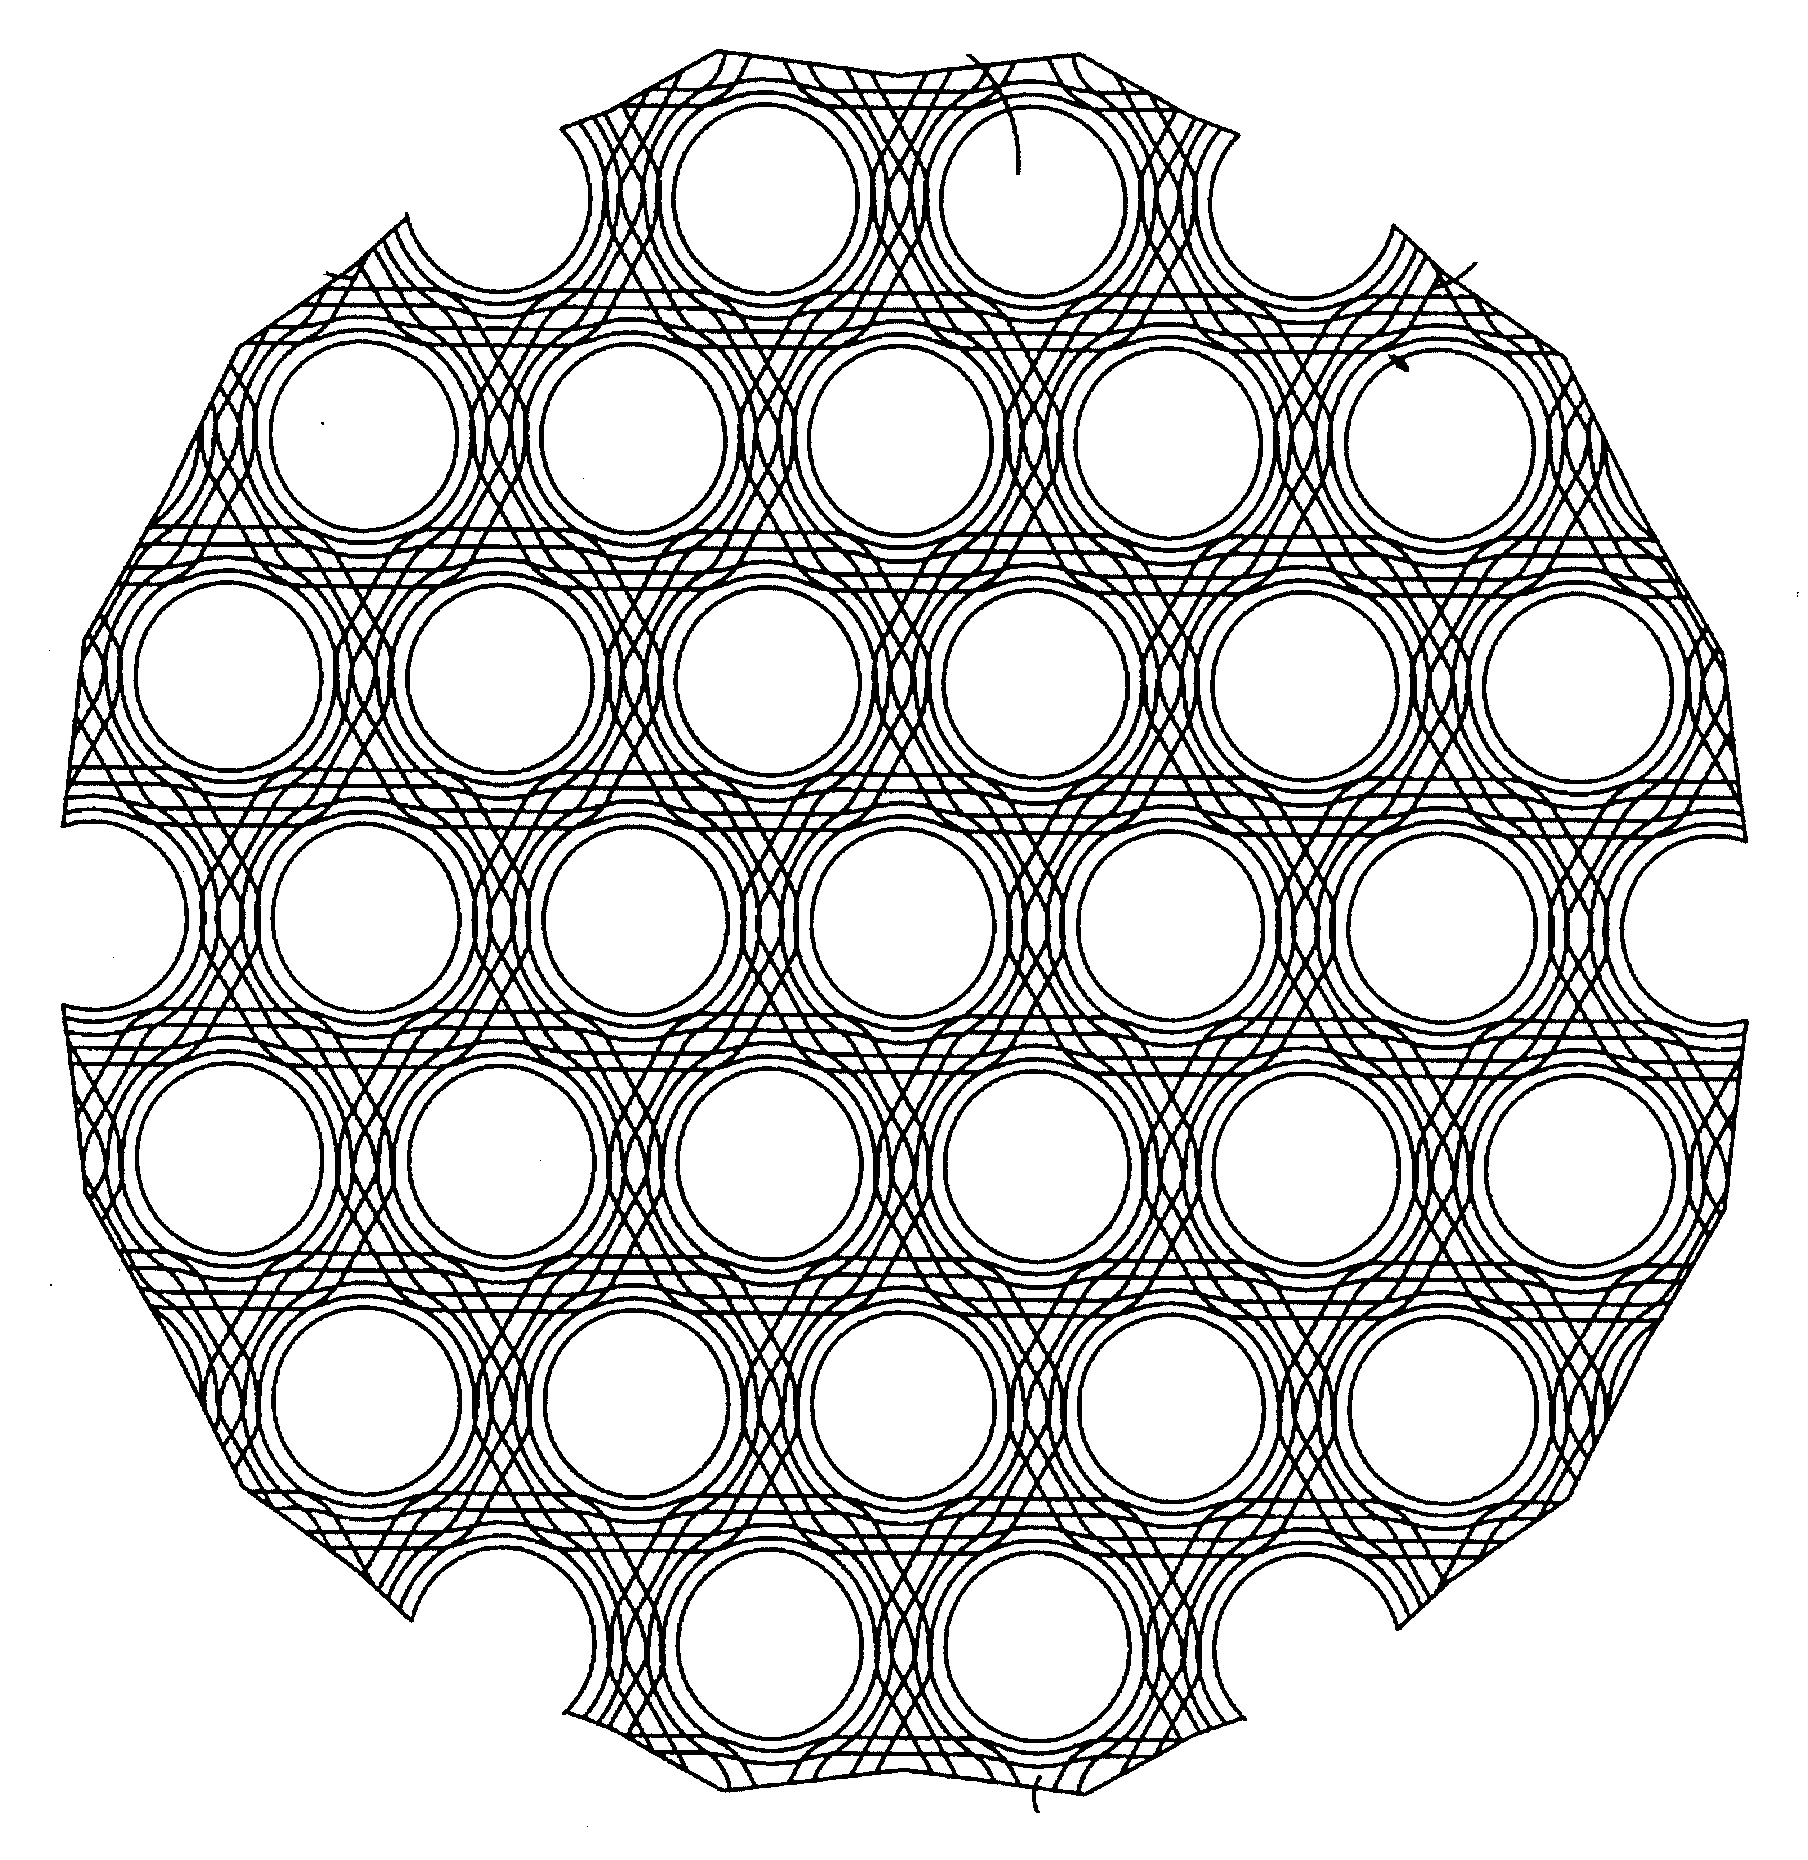
\includegraphics[width=0.5\textwidth]{figs/aperturegrids.png}
    \caption{Distribution of apertures in the grids \cite{aperturegrids}}
    \label{aperturegridspic}
\end{figure}


This papers suggests to create a fourth grid for the magnetic lenses. Since the rays are diverging before the collimating magnets, one expects the aperture of the magnetic lenses to be greater than that of the accelerator grid for any given grid distance $D$. However, thanks to the distribution, it is shown that there exists an upper bound on $D$ such that no jets are lost by diverging and missing the lenses. 

Consider the angle distribution $\theta = \theta_m r/a$ given in section \ref{varyingtheta} and the limits of placed at $-3a/4$ and $+3a/4$ given by the red lines in Figure \ref{RVdistribution}. Then:
\begin{align*}
    \tan \theta & = \tan \theta_m \frac{r}{a} \leq \frac{a}{4} \cdot \dfrac{1}{D} \\
    D & \leq \frac{a}{4 \tan \theta_m \frac{r}{a}}
\end{align*}
which in case for a maximum deviation angle of $\theta_m = 45^{\circ}$, one obtains $D \leq a/4 = 0.31$ mm, comparable to the other grid gaps that are in the range $0.1 to 1$ mm. 


\subsection{Minimal thrust increase from mass considerations}
The added magnets for the considered magnetic field contribute to the total mass $m_t$ with $\Delta m$. The improvement in thrust they give such that at least they "carry" themselves is such that:
\begin{align}
    T = m a \qquad & T' = (m + \Delta m) a \\
    T = F_t T_0 \qquad & T' = F'_t T_0
\end{align}
whence a lower ratio limit is found to be:
\begin{equation}
    \eta = \frac{F'_t}{F_t} = 1 + \frac{\Delta m}{m}
\end{equation}
Consider that the magnetic fields are produced by magnetic lenses (explained in section \ref{magneticlenssection}) by coils with iron cores. The outer and inner radii are $r_o = 0.4$ cm and $r_i = 0.25$ cm and the length of the coil is $L = 10$ cm. Thus, the volume of one magnet lens is at least $V = \pi ((r_o/2)^2 - (r_i/2)^2) L = 0.766$ cm$^3$. Silver is the better material to use for conductors in satellites, but the main mass contribution is given by the iron core (with density $\rho = 7.84$ g/cm$^3$ of the magnets, which gives a contribution up to $\Delta m = 6$ g/lens. 

The total magnetic lenses grid mass roughly sums up to $\Delta m = 6$ kg, reasonable considering the other parts. \cite{dawnmass} Assuming a total space craft mass (without the magnets) of $m = 1,200$ kg (as for the Dawn spacecraft \cite{dawnmass}), one finds:
\begin{equation}
    \eta \approx 1.005
    \label{minimalmassimprovement}
\end{equation}
which means that at 0.5\% increase in thrust suffices. This is a clear argument in favor of using magnetic fields.

\subsection{Front-End Electronics}
The electric devices used to power the magnets have been completely neglected. Together with cabling and other electrical effects, these can alter the magnetic field itself and even deflect the ions. Furthermore, these further increase the energy consumption, thus reducing the space-craft life time. From an electrical engineering perspective, the more elements the ion thruster has, the more difficult to balance the factors in a positive manner.


\section{Simulations}
\label{sectionsimulation}
Coupled with this paper is simulation that demonstrates the trajectories of Xe ions ejected from the ion thruster in real time (\href{https://sigma271.github.io/}{https://sigma271.github.io/}, this version does not accept updates). The authors believe that science should be an open-access platform where any individual can learn and contribute, share and live of the enthusiasm of fellow colleagues and friends. The passion and mission of science is exactly what pushed the authors to study it, hence the developed software will be further adjusted, improved and animated to increase the public awareness of space missions, in particular ion thrusters. The authors invite the readers to contact them for the recent developments and for provinding the scripts.


\subsection{Scales}
Given the small scale of the system, quantities of distance have to be scaled up. $50$ distance units in the simulation will correspond to the radius of the aperture in the setup presented in the problem; $12.5\times 10^{-4}$ meters. Given the high velocities of the Xe ions in the simulation, $8$ distance units per timestep will represent $1.473 \times 10^4$ meters per second. From that, the timestep is \emph{determined} to represent $1.358\times10^{-8}$ seconds. Ideally, the simulation will run the same number of timesteps as the refresh rate of the viewing monitor in Hertz. Furthermore, due to hard limitations in computation, one particle in the simulation will represent multiple Xe ions. For the simulation to be better accessible on old machines, the number of particles on the screen can be tuned up and down.

\begin{figure}[H]
    \centering
    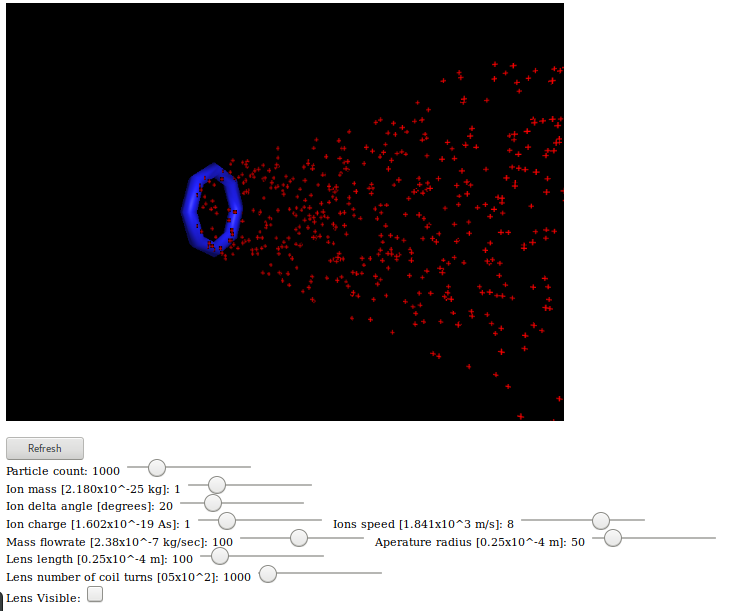
\includegraphics[width=0.5\textwidth]{results/scren.png}
    \caption{Caption}
    \label{fig:my_label}
\end{figure}

\subsection{Assumptions and Approximations}

Several assumption were made in the simulation. The valency of the Xe ions is always taken to be $1$, and no mutual repulsion between the ions were accounted for. The speed at which all Xe move is also taken to be the same for all ions. The uncertainity in the angle is also taken to be uniform. Furthermore, in the preliminary simulation of the magnetic lens that focuses the ions, the magnetic field is only accounted for when ions are inside it. This simplification was made to avoid the complicated edge cases that can happen at the boundaries of the cylinder. The distribution in the positions of the ejected ions was also preliminarily taken to be that of a gaussian distribution, contrary to reality where the ions take the bimodal 2D distribution. 

\subsection{Technical Details}
The simulation was written in Javascript to run on any modern web browsers. Values used in the simulation are chosen so that the entire model is to scale. First, the scale of the distance was establish so that the radius of the aperture in the simulation would fit visibly into the screen; it was decided that 1 unit distance would represent $2.5\times 10^{-0.5}$ m. The scale of the velocity of the ions was then chosen such that 1 unit distance per time-step would represent the velocity: $5.43 \times 10^{-4}$. The time-step could then only be computed to scale so that $1$ time step would correspond to $1.358 \times 10^{-8}$ seconds. 

Taking the mass flow rate of the Xenon ions $2.38 \times 10^{-5}$ kilograms, the corresponding flow rate was then calculated to be $3.232 \times 10^{-13}$ kilograms per time-step. This result was used to keep the flow rate with the ejection of the particles in the simulation consistent and scale-able with the physical results. 

Furthermore, the ions were also made responsive to magnetic fields inducing the lorentz force and changing their trajectory. In particular, parameters of the magnetic lens theorized previously in this treatment were implemented in the simulation. 




\section{Conclusion}
\label{sectionconclusion}
The starting point of this paper is to understand the spatial and velocity distribution of the accelerated ions. Based on previous simulations from literature (on: ionization reactions, charged particle acceleration using grids and their influences), an approximate model was treated: a bimodal 2D Gaussian distribution, which resembles a "donut" hole distribution. This is the best model without explicitly doing the computationally expensive simulation of electron bombardment. The only correction factor of interest was the divergence of the ion beam. Starting from constant jet current density and angle distribution, a more complicated model for the given distribution with linearly increasing angle wrt. to the distance from the centre is theoreticized. 

In order to make the wide angled ions coming outside from the accelerator grid uniform, we introduced the concept of magnetic lens as an another grid after the accelerator grid that converges the ions. We showed that the uniform magnetic field or time-varying magnetic field is not feasible as it brings it own other problems.  Therefore, the concept of non-homogeneous magnetic field was used to make the ion paths uniform. Several assumptions such as non-relativistic ions with no Columb interaction was used. We studied the behavior of ions in non-homogeneous magnetic field and re-derived the Busch equation of focal length. We obtained that focal length of the lens was inversely proportional to the intensity of the magnetic field. Thus, finally focal length of the lens of 2.5m with coil current of 0.0033A with 2500 number of turns was obtained. This shows that ion beams comes out the lens uniform. 

A simulation was also created and coupled with this study. The simulation featured a to-scale treatment of the model, and made it accessible to everyone using web technologies. More work is planned to be done on the simulation in the future. 


An interesting idea is not only to reduce the divergence of the jet beam, but one may also use magnetic fields to steer the rocket. This will be an even slower process, but one may try to deflect all the ions such that their perpendicular momenta to the rocket motion are aligned on a particular direction.

Based on it, it is found that even for a maximum deflection half-angle of 45 degrees, the correction factor decreases only to 91.5\%, hence a theoretical maximal improvement of roughly 10\%.Summarizing, throughout the paper several arguments were brought for and against introducing magnetic fields via magnetic lensing to reduce the ion beam divergence. Since no significant improvement was found without a great deal of technical details and important effects being neglected, it is concluded that this proposal is unpractical. Further investigations are required, together with experimental data.



\newpage
\newpage
\appendix

\section{Distributions and numerics}
\label{appendixnumerical}

To remind the reader, normal distributions of the form:
\begin{equation}
    N_i(\mu,\sigma_i) = \frac{1}{\sqrt{2\pi}\sigma_i} e^{-\dfrac{(x-\mu_i)^2}{2 \sigma_i^2}}
\end{equation}
Normalization constants $\mathcal{N}_i$ are derived such that the mixture probability distribution for the bimodal (two Gaussians) with mixing parameter $p$ obeys:
\begin{align*}
    1 & = \int_{-a}^{+a} f(x)dx = \\
    & = \int_{-a}^{+a} (p \mathcal{N}_1 N_1 + (1-p) \mathcal{N}_2 N_2)dx \numberthis{}
\end{align*}
Here $p =0.5 $, i.e. equally weighted distributions. One existing condition for bimodal distribution is that:
\begin{equation}
    |\mu_1 - \mu_2| > |\sigma_1 + \sigma_2|
\end{equation}
which holds for the considered case of $\mu_{1,2} = \pm a/4$ with the same standard deviation $\sigma_1 = \sigma_2=\sigma = a/4$.

\subsection{Distribution function and constant correction factor}
Since the Gaussians are extended over the whole real axis and in this approach one cuts it to a finite interval, the normalization constants $\mathcal{N}_i$ are needed to upscale them back (Note that $\mathcal{N}_1 = \mathcal{N}_2$ due to the symmetry of the Gaussian distribution):
\begin{align*}
    & \mathcal{N}_i  = \dfrac{\int_{-\infty}^{+\infty} N(\mu_i, \sigma)}{\int_{-a}^{+a} N(\mu_i, \sigma)} = \dfrac{1}{\int_{-a}^{+a} N(\frac{a}{4}, \frac{a}{4})} =\\
    & =  \dfrac{8}{\erf\left( \dfrac{3}{\sqrt{2}}\right) + \erf\left( \dfrac{5}{\sqrt{2}}\right)} \approx \dfrac{1}{0.249} = 4 \cdot 0.996 \numberthis
    \label{approxexample}
\end{align*}

Moreover, since two Gaussians are used, a factor of a half comes up front, yielding:
\begin{equation}
    f(x) = \dfrac{4}{a} \sqrt{\dfrac{2}{\pi}}\left[ e^{-\dfrac{(4x+a)^2}{2 a^2}} + e^{-\dfrac{(4x-a)^2}{2 a^2}} \right]
    \label{finaldistributionappendix}
\end{equation}

As an example, the numerical term in the correction factor of equation \ref{constantthetasolution} comes from an integration beast:
\begin{align*}
 & 2 \cdot 0.4971097 = \int_{-a}^{+a} r f(r) =\\ & \dfrac{e^{25/2} \sqrt{2\pi} 
  \left( erf(\frac{3}{\sqrt{2}}) + erf(\frac{5}{\sqrt{2}})  \right) + 2 - 2 e^8}{4 e^{25/2} \sqrt{2\pi}} \numberthis 
\end{align*}

\subsection{Correction factor for radius varying angle}
\label{appendixnumericalb}
The integral of \ref{complicatedintegral} requires a Taylor expansion of the cosine as:
\begin{equation}
    \cos \alpha \dfrac{\pi r}{2 a} = 1 - \dfrac{1}{2!} \left( \alpha \dfrac{\pi r}{2 a} \right)^2 + \dfrac{1}{4!} \left( \alpha \dfrac{\pi r}{2 a} \right)^4 + \hdots
\end{equation}
Truncating after three terms only (since the third contribution is of the order $10^{-6}$ yields after integration:
\begin{equation}
    F_t(\alpha)  = 2 ( 0.497 - \dfrac{0.121647}{2!} \alpha ^2 + \dfrac{0.046183}{4!} \alpha^4)
\end{equation}

\subsection{Independent Random Variables}
\label{randomvariables}
Note that equation \ref{finaldistributionappendix} can be slightly misleading: it is meant here that the mean $\mu$ and variance $\sigma$ (which are two independent variables) can be expressed as via the aperture radius $a$ (and the function becomes function of only one variable). In the numerical computations, first each independent Gaussian is computed and then they are summed up. Otherwise, one ends up with only one Gaussian. Probabilistically, one should not confuse the mixture probability with the sum of two Gaussians.

\onecolumn
\section{Javascript simulation, HTML script and Python script}

\lstinputlisting[language=Java]{results/script.js}

\lstinputlisting[language=HTML]{results/index.html}

\lstinputlisting[language=Python]{physicsproject.py}

\twocolumn

\newpage

\bibliographystyle{unsrt}
\bibliography{biblio}

All Website were accessed on November 11th and 12th, 2017
\end{document}
